\section{Design Aeronáutico}

A área de Design Aeronáutico desempenha um papel fundamental na equipe, sendo responsável por analisar, selecionar e integrar os componentes propulsivos, estruturais e energéticos. Isso engloba o estudo de motores, hélices, baterias, análises estruturais e controladores de velocidade eletrônicos, garantindo que todos os sistemas funcionem em sincronia, visando o maior desempenho possível.

\subsection*{Objetivo}

O projeto consiste na construção de um drone teórico, com base na missão previamente apresentada. Será necessário selecionar os componentes a partir de parâmetros definidos, apresentando justificativas técnicas para as escolhas e análises que confirmem sua viabilidade. A proposta exige uma avaliação criteriosa dos parâmetros de cada componente, a fim de determinar a melhor escolha para o cenário proposto.

A escolha dos componentes será dividida em três categorias principais:
\begin{enumerate}
    \item Frame da Aeronave
    \item Componentes Propulsivos
    \item Bateria
\end{enumerate}

\subsubsection*{Frame da Aeronave}

O frame deverá ser modelado utilizando um software de CAD, como CATIA, SolidWorks, Fusion 360 ou similares. É necessário realizar análises estruturais teóricas e simulações em softwares apropriados. Em termos dimensionais, o frame deve possuir entre 150 mm e 500 mm de distância entre eixos, o que geralmente corresponde à distância entre os centros de motores opostos, com braços dispostos a 90° entre si, conforme a ilustração a seguir:

    \begin{figure}[H]
    \centering
    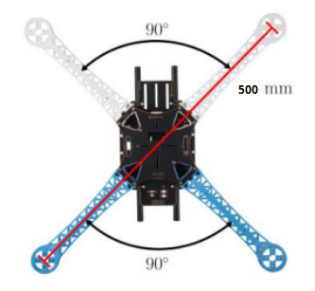
\includegraphics[width=0.5\linewidth]{Editáveis/image.png}
    \label{fig:enter-label}
\end{figure}

A estrutura do frame deve ser composta por quatro partes principais:
\begin{itemize}
    \item Hastes
    \item Trens de pouso
    \item Placa central superior
    \item Placa central inferior
\end{itemize}

\subsubsection*{Componentes Propulsivos}

Nesta seção serão analisados os motores e hélices necessários para alcançar o desempenho desejado.

\textbf{Motores:}  
\begin{itemize}
    \item A aeronave deve possuir 4 rotores idênticos do tipo \textit{brushless}, com faixa de operação entre 700KV e 2000KV.
    \item Devem ser avaliadas propriedades físicas, características de desempenho e documentação técnica dos fabricantes.
\end{itemize}

\textbf{Hélices:}  
\begin{itemize}
    \item Avaliar o diâmetro e o passo das hélices, considerando sua influência no desempenho, empuxo e consumo energético.
    \item Justificar a escolha com base em gráficos de desempenho e eficiência.
\end{itemize}

\subsubsection*{Bateria}

A bateria é um dos principais elementos do sistema energético do drone, influenciando diretamente no tempo de voo e na operação dos sistemas embarcados.

\begin{itemize}
    \item Avaliar parâmetros como capacidade, tensão, peso, eficiência energética e compatibilidade com os demais componentes.
    \item A bateria escolhida deve fornecer autonomia de pelo menos 15 minutos em voo estacionário (\textit{hover}).
\end{itemize}

\subsubsection*{Etapa Final – Relatório}

Durante o desenvolvimento do projeto, é indispensável documentar todas as etapas com clareza e organização. A justificativa técnica para cada escolha deve ser bem fundamentada com base em dados, análises e simulações.

\textbf{O relatório final deve conter:}
\begin{itemize}
    \item Justificativas técnicas para cada componente selecionado
    \item Comparativos e análises entre diferentes opções
    \item Cálculos e parâmetros relevantes utilizados na seleção
    \item Diagramas, imagens ou tabelas que ajudem a ilustrar as decisões tomadas
    \item Conclusões sobre a viabilidade do projeto em relação à missão proposta
\end{itemize}
